\let\negmedspace\undefined
\let\negthickspace\undefined
\documentclass[journal]{IEEEtran}
\usepackage[a5paper, margin=10mm, onecolumn]{geometry}
%\usepackage{lmodern} 
\usepackage{tfrupee} 

\setlength{\headheight}{1cm} 
\setlength{\headsep}{0mm}     

\usepackage{gvv-book}
\usepackage{gvv}
\usepackage{cite}
\usepackage{amsmath,amssymb,amsfonts,amsthm}
\usepackage{algorithmic}
\usepackage{graphicx}
\usepackage{textcomp}
\usepackage{xcolor}
\usepackage{txfonts}
\usepackage{listings}
\usepackage{enumitem}
\usepackage{mathtools}
\usepackage{gensymb}
\usepackage{comment}
\usepackage[breaklinks=true]{hyperref}
\usepackage{tkz-euclide} 
\usepackage{listings}                                        
\def\inputGnumericTable{}                                 
\usepackage[latin1]{inputenc}                                
\usepackage{color}                                            
\usepackage{array}                                            
\usepackage{longtable}                                       
\usepackage{calc}                                             
\usepackage{multirow}                                         
\usepackage{hhline}                                           
\usepackage{ifthen}                                           
\usepackage{lscape}

\begin{document}

\bibliographystyle{IEEEtran}
\vspace{3cm}

\title{8.2.37}
\author{AI25BTECH11003 - Bhavesh Gaikwad}
{\let\newpage\relax\maketitle}

\renewcommand{\thefigure}{\theenumi}
\renewcommand{\thetable}{\theenumi}
\setlength{\intextsep}{10pt} 


\numberwithin{equation}{enumi}
\numberwithin{figure}{enumi}
\renewcommand{\thetable}{\theenumi}


\textbf{Question}: Find the equation of the conic, that satisfies the given conditions.\\
vertex (-3, 0), directrix x + 5 = 0.\\

\textbf{Solution:}\\
Given:
\begin{itemize}
\item Vertex: $\vec{V_o} = \myvec{-3 \\ 0}$
\item Directrix: $x + 5 = 0$, which gives us $\vec{n}^\top\vec{x} = c$ where $\vec{n} = \myvec{1 \\ 0}$ and $c = -5$
\end{itemize}

The general matrix equation of a conic is:
\begin{equation}
\vec{x}^\top\vec{V}\vec{x} + 2\vec{u}^\top\vec{x} + f = 0
\end{equation}

where the matrices are defined as:
\begin{align}
\vec{V} &= \norm{\vec{n}}^2\vec{I} - e^2(\vec{n}\vec{n}^\top) \\
\vec{u} &= (ce^2)\vec{n} - \norm{\vec{n}}^2\vec{F} \\
f &= \norm{\vec{n}}^2\norm{\vec{F}}^2 - c^2e^2
\end{align}

For a vertex at $(-3, 0)$ and using the vertex-focus-directrix geometry, the focus $\vec{F}$ is at:
\begin{equation}
\vec{F} = \myvec{-3 + 2e \\ 0}
\end{equation}

\newpage

\textbf{Case 1: $e < 1$} (Ellipse)\\
Let $e = \frac{1}{2}$

\textbf{Parameters:}
\begin{itemize}
\item $\vec{n} = \myvec{1 \\ 0}$, $c = -5$, $e = \frac{1}{2}$
\item $\vec{F} = \myvec{-2 \\ 0}$
\item $||\vec{n}||^2 = 1$, $||\vec{F}||^2 = 4$
\end{itemize}

Matrix Calculation:\\
\begin{align}
\vec{V} &= \myvec{1 & 0 \\ 0 & 1} - \frac{1}{4}\myvec{1 & 0 \\ 0 & 0} = \myvec{3/4 & 0 \\ 0 & 1}
\end{align}

\begin{align}
\vec{u} &= \frac{-5}{4}\myvec{1 \\ 0} - \myvec{-2 \\ 0} = \myvec{3/4 \\ 0}
\end{align}

\begin{align}
f &= 4 - \frac{25}{4} = -\frac{9}{4}
\end{align}

\bigskip

Putting Values of $\vec{V}, \, \vec{u}$, f in Equation 0.1, we get
\begin{equation}
\vec{x}^\top\myvec{3 & 0 \\ 0 & 4}\vec{x} + \myvec{6 & 0}\vec{x} - 9 = 0
\end{equation}



\newpage

\textbf{Case 2: $e = 1$} (Parabola)\\
\textbf{Parameters:}
\begin{itemize}
\item $\vec{n} = \myvec{1 \\ 0}$, $c = -5$, $e = 1$
\item $\vec{F} = \myvec{-1 \\ 0}$
\item $||\vec{F}||^2 = 1$
\end{itemize}

\bigskip

Matrix Calculation:
\begin{align}
\vec{V} &= \myvec{1 & 0 \\ 0 & 1} - \myvec{1 & 0 \\ 0 & 0} = \myvec{0 & 0 \\ 0 & 1}
\end{align}

\begin{align}
\vec{u} &= -5\myvec{1 \\ 0} - \myvec{-1 \\ 0} = \myvec{-4 \\ 0}
\end{align}

\begin{align}
f &= 1 - 25 = -24
\end{align}

Putting Values of $\vec{V}, \, \vec{u}$, f in Equation 0.1, we get
\begin{equation}
\vec{x}^\top\myvec{0 & 0 \\ 0 & 1}\vec{x} + \myvec{-8 & 0}\vec{x} - 24 = 0
\end{equation}


\newpage

\textbf{Case 3: $e > 1$} (Hyperbola)\\
Let $e = \frac{3}{2}$

\textbf{Parameters:}
\begin{itemize}
\item $\vec{n} = \myvec{1 \\ 0}$, $c = -5$, $e = \frac{3}{2}$
\item $\vec{F} = \myvec{0 \\ 0}$
\item $||\vec{F}||^2 = 0$
\end{itemize}

\bigskip

Matrix Calculation:
\begin{align}
\vec{V} &= \myvec{1 & 0 \\ 0 & 1} - \frac{9}{4}\myvec{1 & 0 \\ 0 & 0} = \myvec{-5/4 & 0 \\ 0 & 1}
\end{align}

\begin{align}
\vec{u} &= \frac{-45}{4}\myvec{1 \\ 0} - \myvec{0 \\ 0} = \myvec{-45/4 \\ 0}
\end{align}

\begin{align}
f &= 0 - \frac{225}{4} = -\frac{225}{4}
\end{align}

Putting Values of $\vec{V}, \, \vec{u}$, f in Equation 0.1, we get
\begin{equation}
\vec{x}^\top\myvec{5 & 0 \\ 0 & -4}\vec{x} + \myvec{90 & 0}\vec{x} + 225 = 0
\end{equation}


\bigskip

Therefore, The Possible conics with the vertex at (-3,0) and Directrix as x+5=0 are\\
$$\vec{x}^\top\myvec{3 & 0 \\ 0 & 4}\vec{x} + \myvec{6 & 0}\vec{x} = 9$$
$$\vec{x}^\top\myvec{0 & 0 \\ 0 & 1}\vec{x} + \myvec{-8 & 0}\vec{x} = 24$$
$$\vec{x}^\top\myvec{5 & 0 \\ 0 & -4}\vec{x} + \myvec{90 & 0}\vec{x} + 225 = 0$$


\begin{figure}
    \centering
    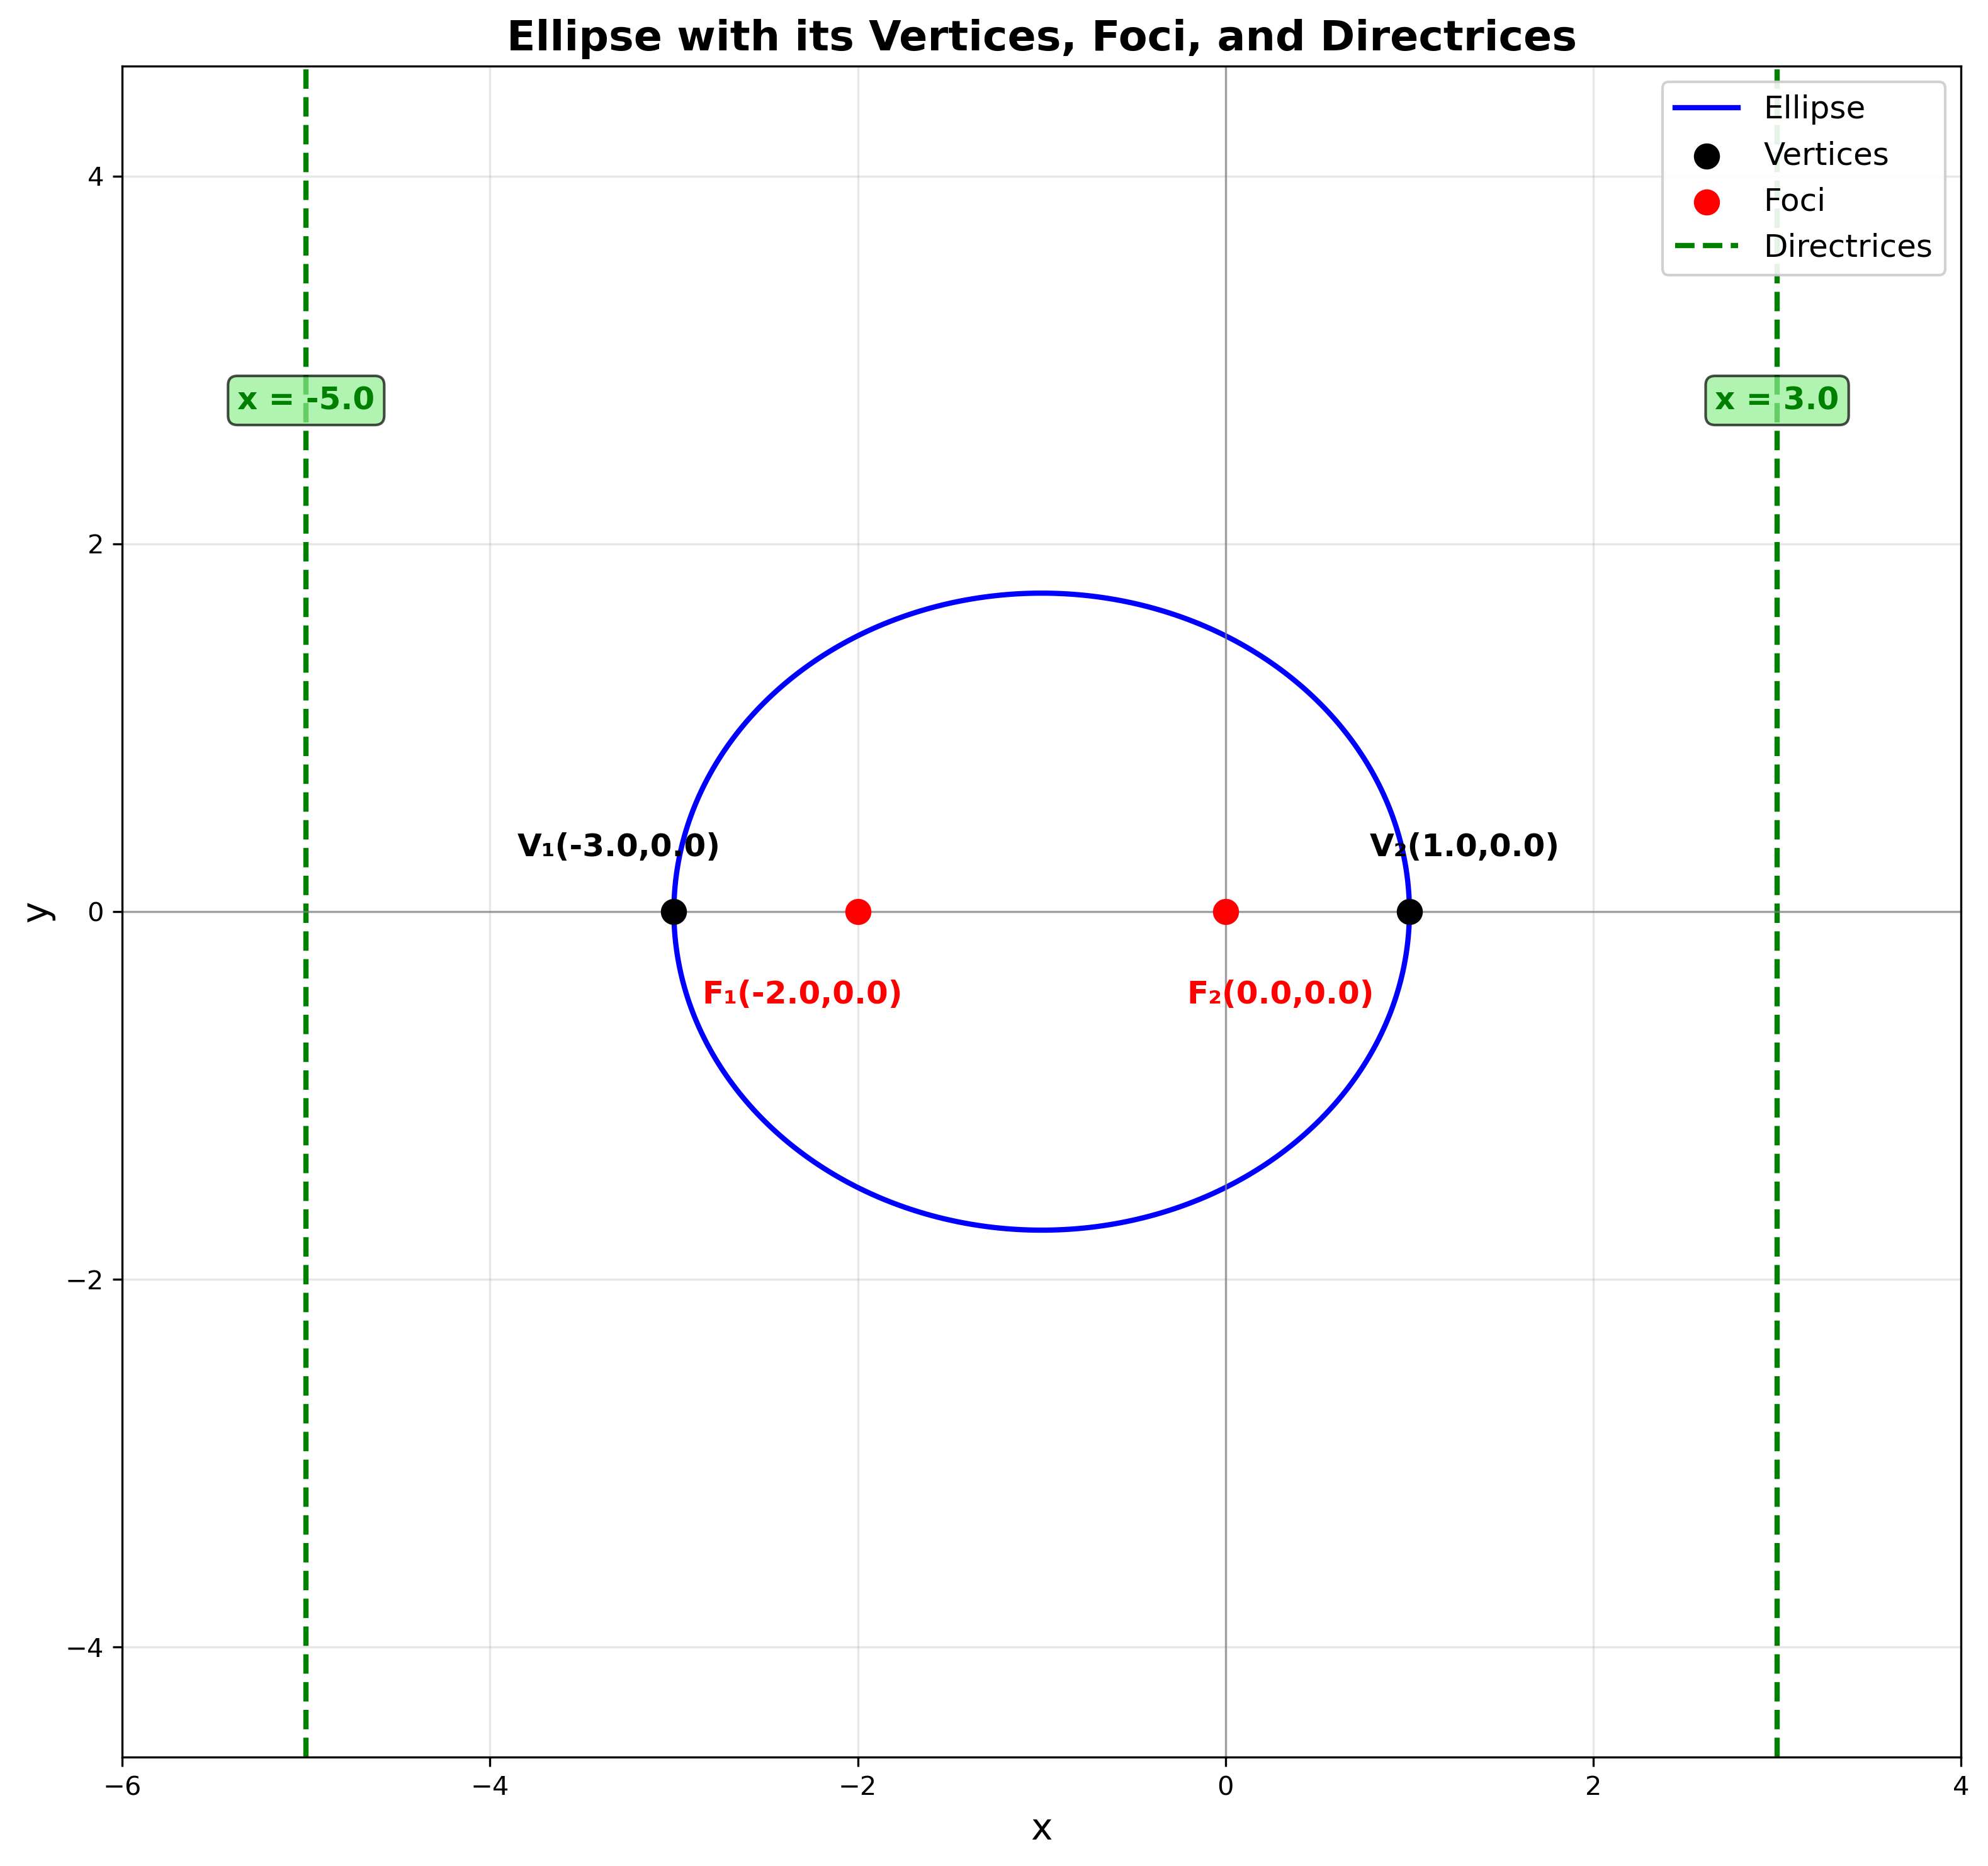
\includegraphics[width=\columnwidth]{figs/fig1.png}
    \caption{Ellipse}
    \label{fig:figs/fig1.png}
\end{figure}

\begin{figure}
    \centering
    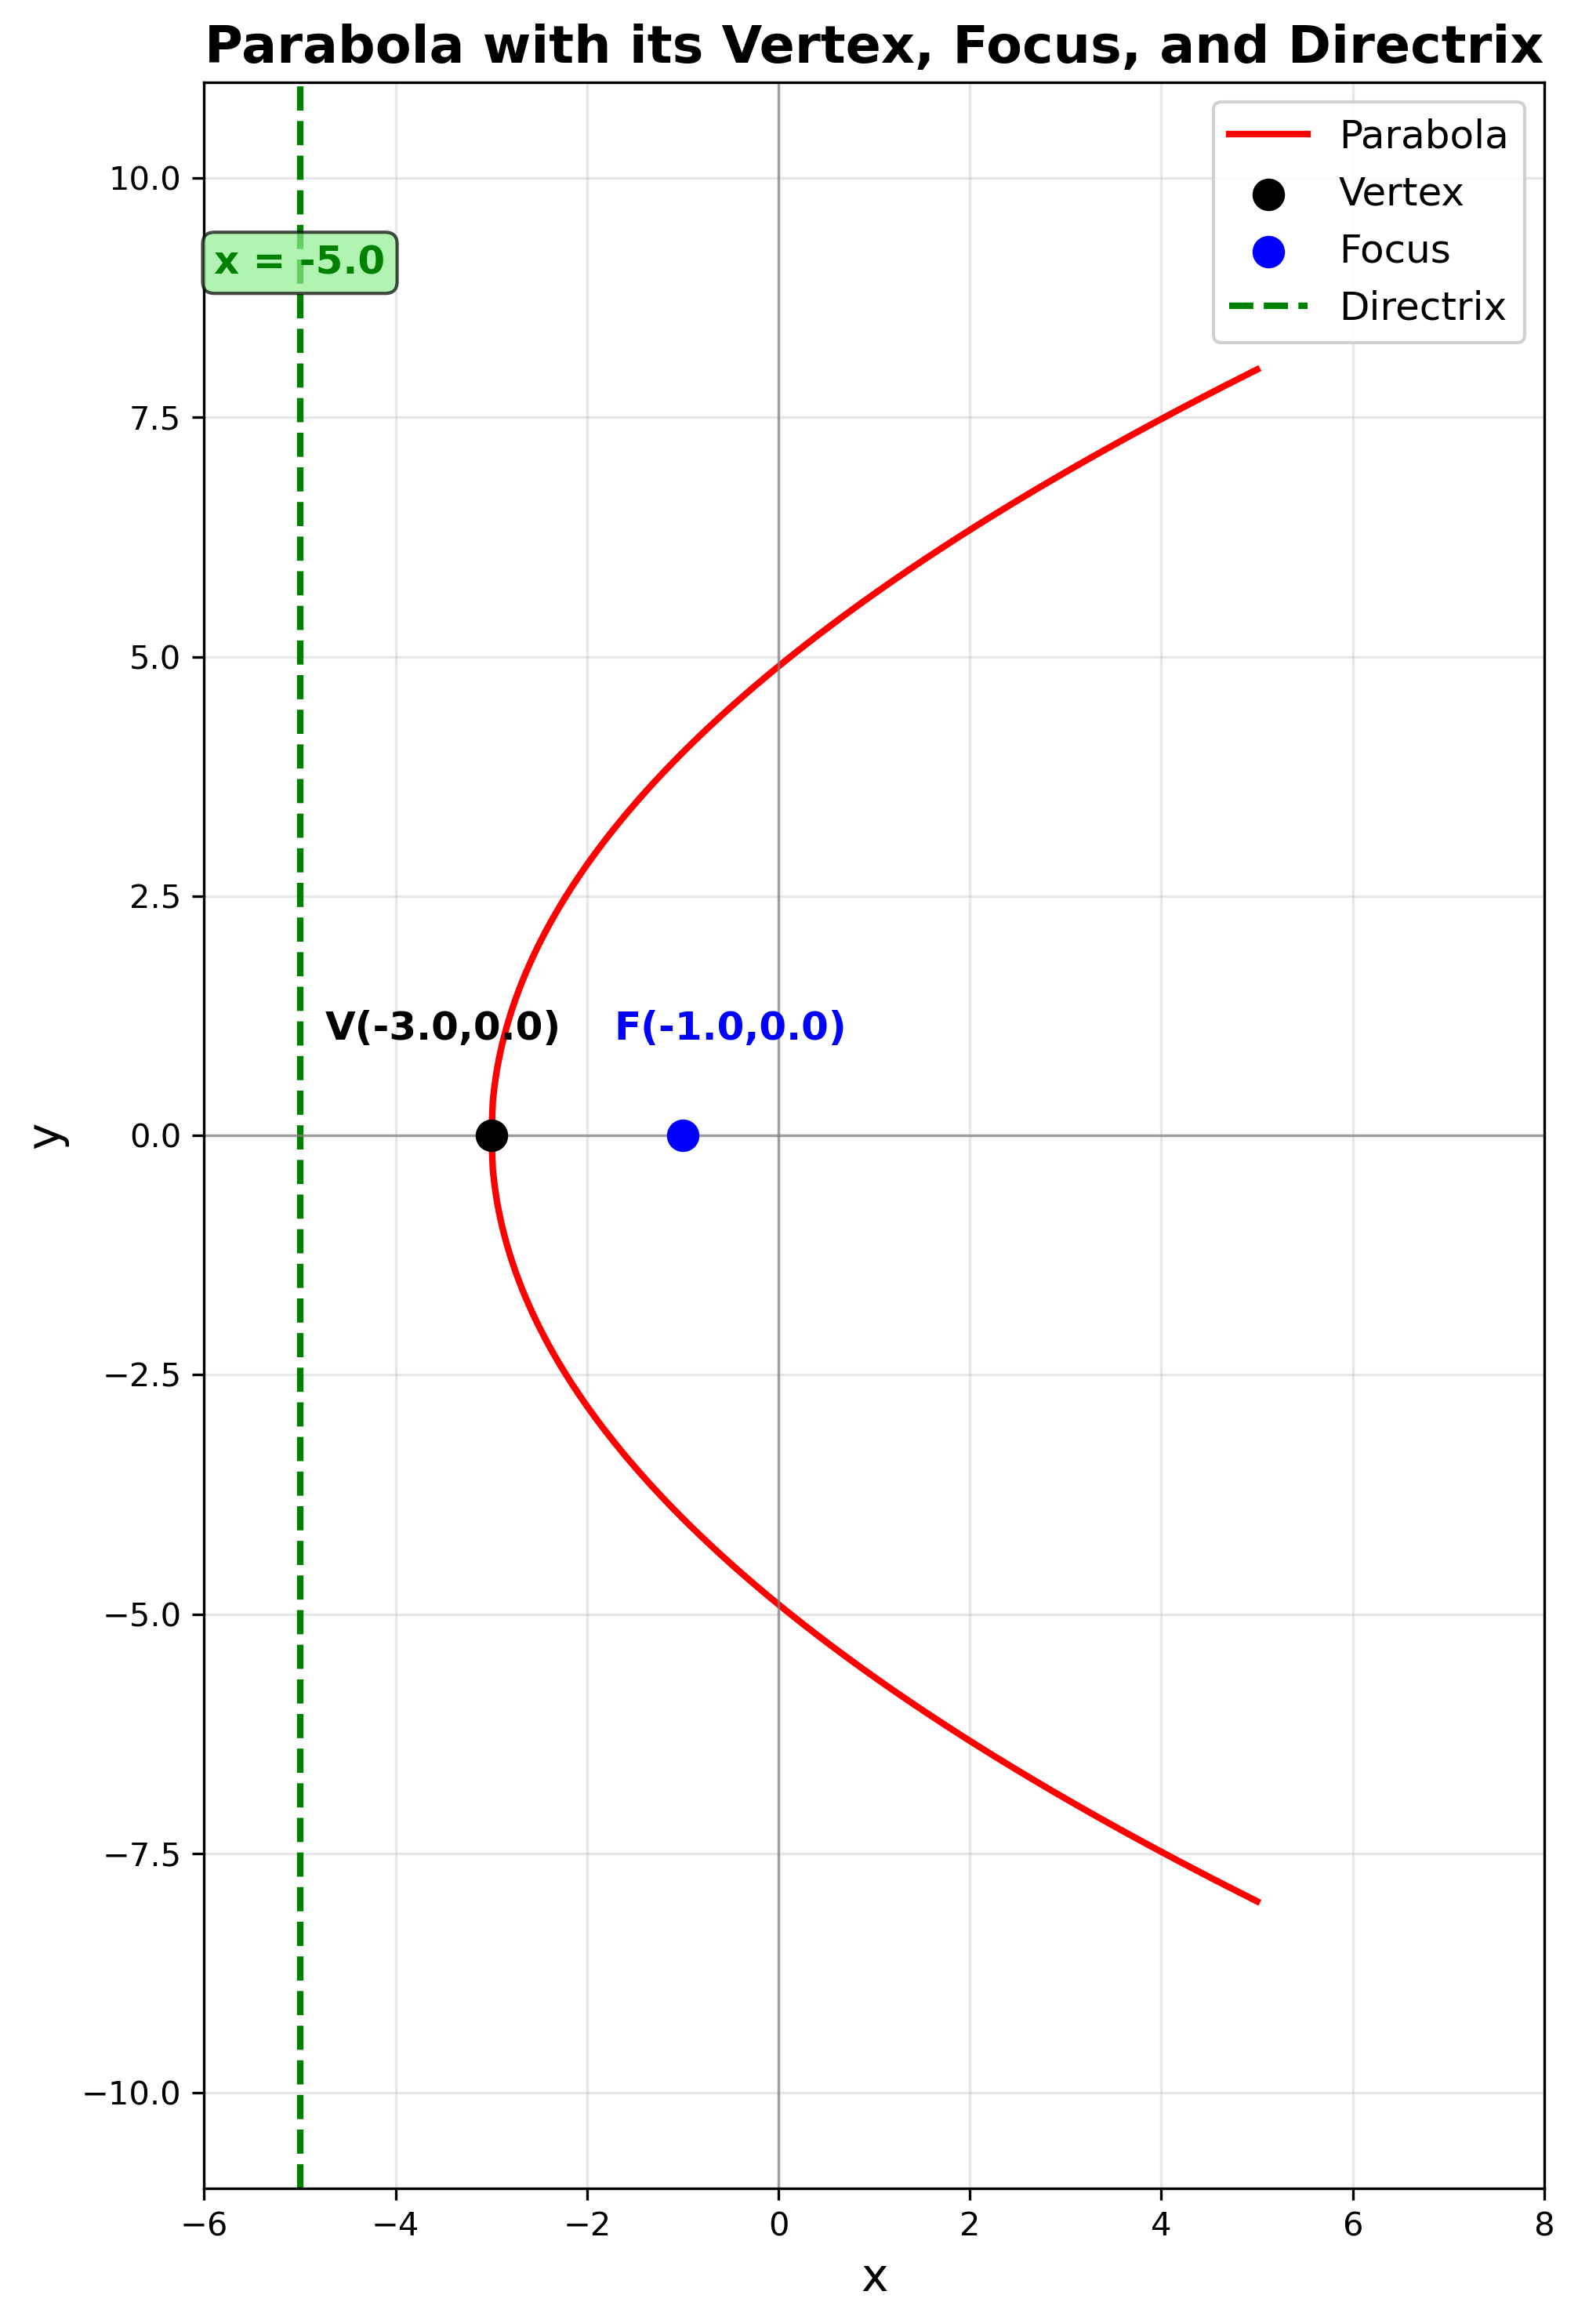
\includegraphics[width=\columnwidth]{figs/fig2.png}
    \caption{Parabola}
    \label{fig:figs/fig2.png}
\end{figure}

\begin{figure}
    \centering
    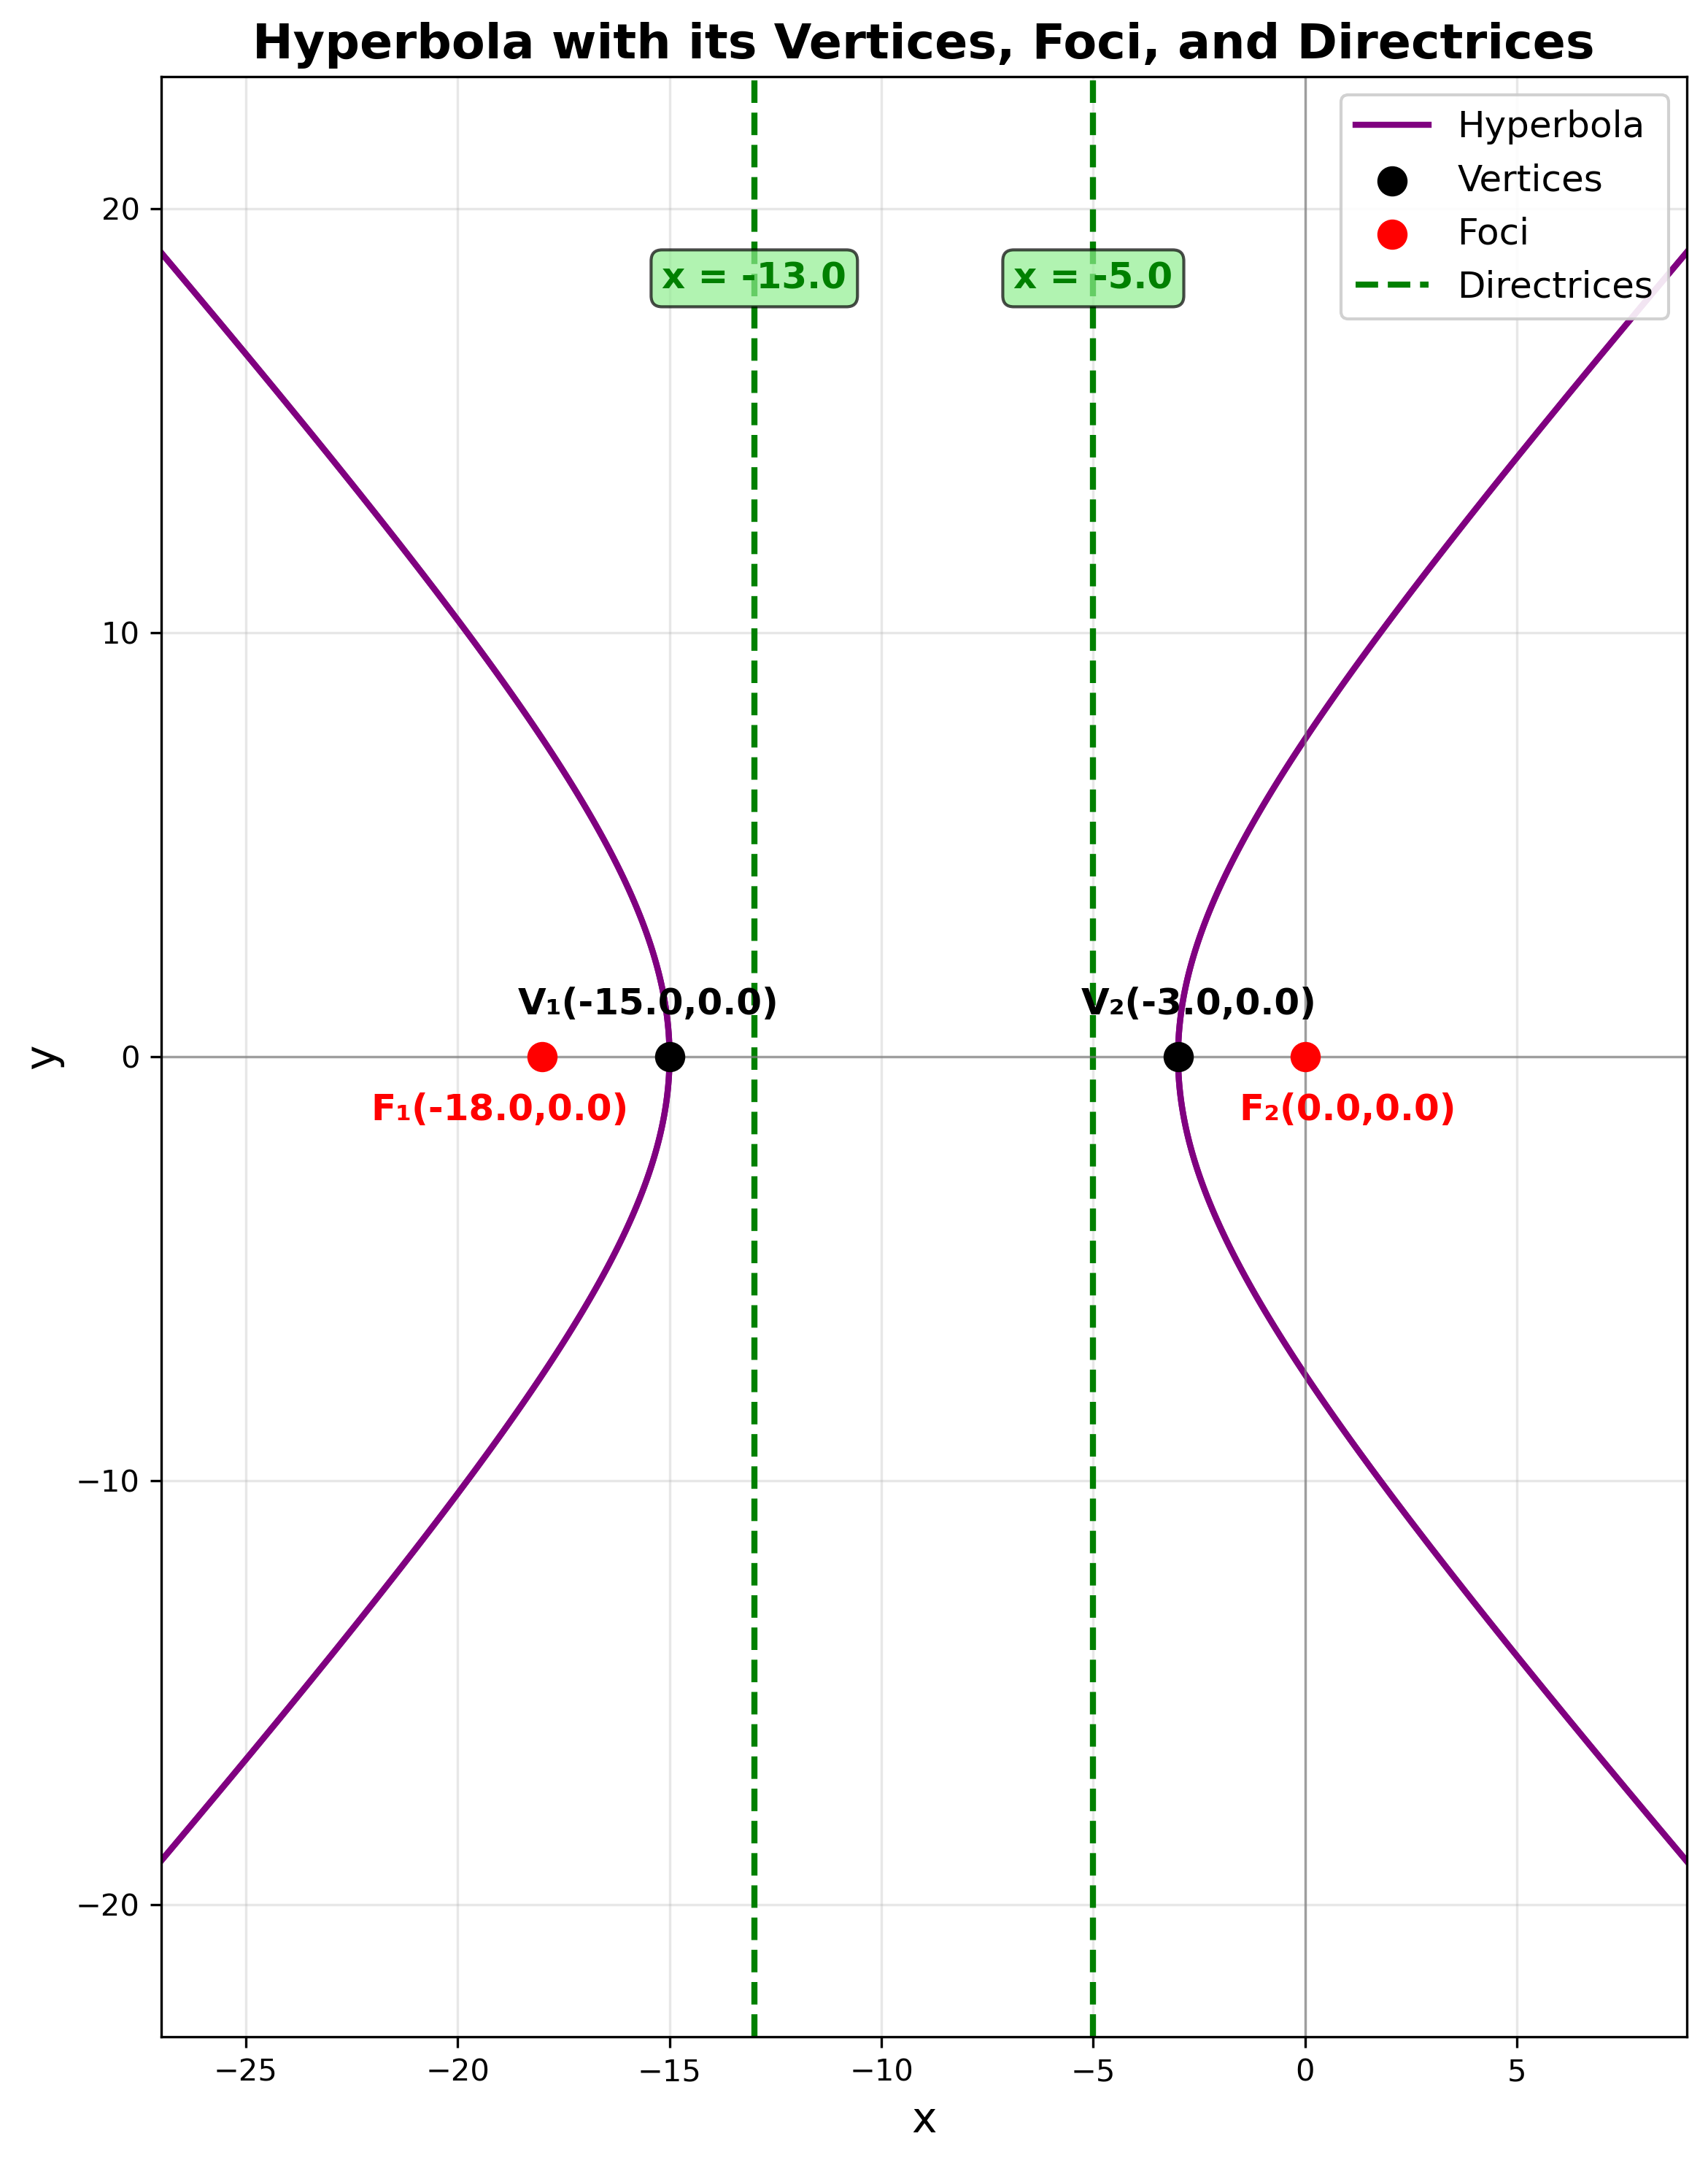
\includegraphics[width=\columnwidth]{figs/fig3.png}
    \caption{Hyperbola}
    \label{fig:figs/fig3.png}
\end{figure}

\end{document}  
